\documentclass[english]{beamer}

\usepackage{tikz}

\usetikzlibrary {arrows.meta,decorations.text, decorations.pathmorphing, decorations.pathreplacing, decorations.shapes,
}

\usepackage{amsmath}
\usepackage{amsfonts}
\usepackage{amssymb}
\usepackage{eurosym}
\usepackage{mathtools}
\usepackage{float}
\usepackage{xfrac}
\usepackage{mathrsfs} 



\usepackage[
  backend=biber,
  style=alphabetic,
  sorting=nty,
  maxbibnames=99,
  url=false,  % Exclude URLs
  % issn = false
  %doi=false,   % Exclude DOIs
  %isbn=false
]{biblatex}

\addbibresource{sample.bib}

\newcommand{\nc}{\newcommand}
\newcommand{\cN}{\mathcal{N}}
\newcommand{\cG}{\mathcal{G}}
\newcommand{\cE}{\mathcal{E}}
\newcommand{\cW}{\mathcal{W}}
\newcommand{\cD}{\mathcal{D}}
\nc{\cV}{\mathcal{V}}
\nc{\cT}{\mathcal{T}}
\nc{\bE}{\mathbb{E}}


%parameters and variables
\nc{\PV}{\mathcal{PV}}
\nc{\HL}{\mathcal{H}^L}
\nc{\PL}{\mathcal{P}^L}
\nc{\WW}{\mathcal{W}}
\nc{\ns}{\text{ns}}
\nc{\nw}{\text{nw}}
\nc{\nh}{\text{nh}}
\nc{\PP}{\text{P}}
\nc{\HH}{\text{H}}
\nc{\HS}{\text{H}^S}
\nc{\CG}{C_{\Sigma}^{\text{Gauss}}}
\usetikzlibrary{shapes,arrows}

\tikzstyle{block} = [draw, fill=blue!20, rectangle, minimum height=4em, minimum width=6em]
\tikzstyle{circleblock} = [draw, fill=red!20, circle, minimum height=4em]
\tikzstyle{line} = [draw, -latex]


\title[MTA Competition]{Capacity Expansion of the Energy Grid: Coupled Scenario Generation and Time Aggregation}

\author[G.R., B.U.]{Gabor Riccardi, Bianca Urso}

\institute{University of Pavia (UniPV) \\ Istituto Universitario di Studi Superiori (IUSS)}

\begin{document}

% Generate title page
{
\setbeamertemplate{footline}{} 
\begin{frame}
  \titlepage
\end{frame}
}
\addtocounter{framenumber}{-1}



\begin{frame}{Introduction}

    %TODO: use a cuter itemize (what about penguins?)
    %TODO: insert a meme
  
  \end{frame}
  
  \begin{frame}{Workflow}
  \frametitle{Workflow}
  \begin{center}
    \resizebox{0.5\textwidth}{!}{
    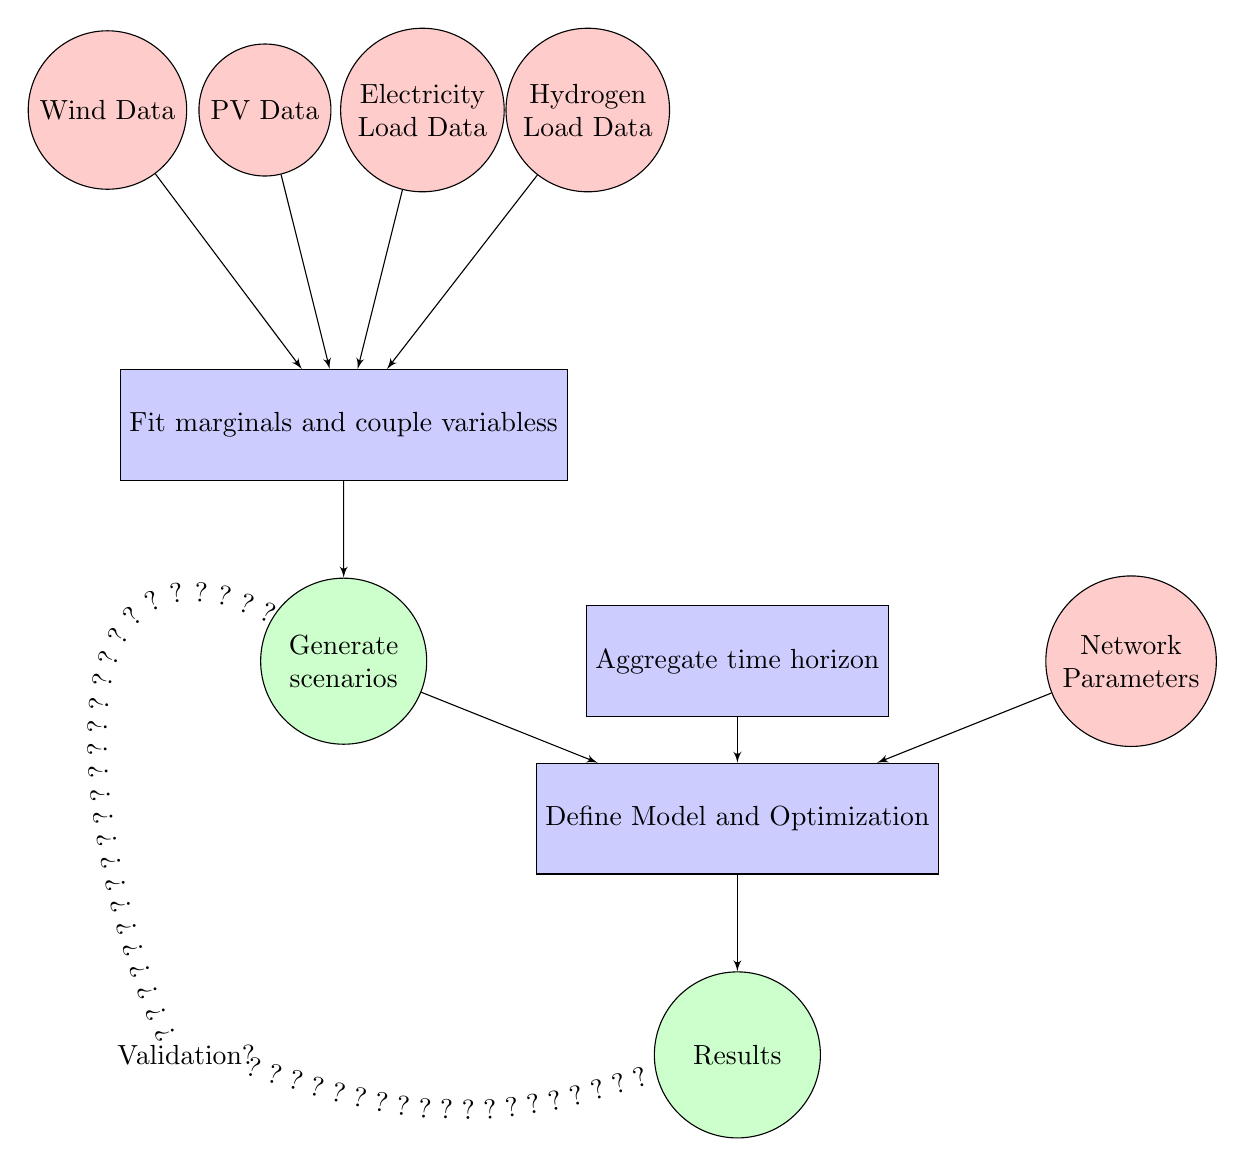
\begin{tikzpicture}[node distance=2cm, auto, >=stealth]
    % Define styles for blocks and lines
    \tikzstyle{circleblock} = [draw, fill=red!20, circle, minimum height=4em, minimum width=4em, text centered]
    \tikzstyle{block} = [draw, fill=blue!20, rectangle, minimum height=4em, minimum width=6em]
    \tikzstyle{block2} = [draw, fill=green!20, circle, minimum height=4em, minimum width=6em]
    \tikzstyle{line} = [draw, -latex']
    
    % Place nodes
    \node [circleblock] (winddata) {Wind Data};
    \node [circleblock, right of = winddata, xshift= 0cm] (PVdata) {PV Data}; % Added xshift for spacing
    \node [circleblock, right of = PVdata, xshift=2cm] (Ploaddata) [align=center,midway] {Electricity  \\ Load Data}; % Added xshift for spacing
    \node [circleblock, right of = Ploaddata, xshift=4.1cm] (Hloaddata) [align=center,midway] {Hydrogen  \\ Load Data}; % Added xshift for spacing
  
    \node [block, below of = PVdata, yshift=-2cm,xshift=1cm] (Fitdata) {Fit marginals and couple variabless};
    \node [block2, below of = Fitdata, yshift=-5cm,xshift=3cm] (SG)  [align=center,midway] {Generate  \\ scenarios}; % Adjusted yshift for spacinga
    \node [block, right of = SG,xshift=3cm] (TA) {Aggregate time horizon};
    \node [block, below of = TA] (OPT) {Define Model and Optimization};
    \node [circleblock, right of = TA, xshift=11cm,yshift=-7cm] (Param) [align=center,midway] {Network  \\ Parameters};
  
    \node [block2, below of = OPT,yshift=-1cm] (RES) {Results};
    \node [left of = RES, xshift = -5cm] (VAL) {Validation?};
    % Draw edges
    \path [line] (winddata) -- (Fitdata);
    \path [line] (PVdata) -- (Fitdata);
    \path [line] (Hloaddata) -- (Fitdata);
    \path [line] (Ploaddata) -- (Fitdata);
    \path [line] (Fitdata) -- (SG);
    \path [line] (SG) -- (OPT);
    \path [line] (TA) -- (OPT);
    \path [line] (Param) -- (OPT);
    \path [line] (OPT) -- (RES);
    \draw decorate [{Stealth[red]-},decoration={text along path, text=    ? ? ? ? ? ? ? ? ? ? ? ? ? ? ? ? ? ? ? ? ? ? ? ? ? ? ? ? ? }] {(VAL) .. controls (4,-13) and (5,-13) .. (RES)};
    \draw decorate [{Stealth[red]-},decoration={text along path, text=    ? ? ? ? ? ? ? ? ? ? ? ? ? ? ? ? ? ? ? ? ? ? ? ? ? ? ? ? ? }] {(VAL) .. controls (0,-10) and (-1,-5) .. (SG)};
    \end{tikzpicture}
    }
    \end{center}
    
  \end{frame}
  
  \section{Model Description}
  
  \begin{frame}{Model 1}
  
  %We model the problem as a Capacity Expansion Problem (CEP), that is a two stage stochastic program: \pause
  We consider a two stage stochastic program consisting of a Capacity Expansion Problem (CEP) and an Economic Dispatch (ED) problem:
    \begin{align*}
      \min_{x} \; & c'x + \bE_{\omega}\left[\cV(x,\omega)\right] \\  \tag{CEP}
      s.t. \;   \quad  & 0 \leq x_{n,g} \leq X_{n,g}
    \end{align*}
    \begin{itemize}
      \pause
      \item The first stage determines the capacity expansion (\(x\)) for each generator \(g \in \cG \) and network component.\pause
      \item The second stage solves the Economic Dispatch (ED) in function of the expanded capacities \(x\) and the scenario \(\omega\), yielding \(\cV(x,\omega)\) as solution.
    \end{itemize}
  \end{frame}
  
  
  
  
  \begin{frame}{Economic Dispatch (ED) model \; \only<2>{\textcolor{red}{Scary Slide}}}
    \pause \pause
  
  
    % For a fixed scenarios \(\omega = (\mathcal{PV}, \mathcal{W}, \mathcal{D})\) comprising of respectively solar power, wind power and loads,  \pause
    % let \: \( y_{\omega} = (Pf_{\omega},Hf_{\omega},H_{\omega}, s)'\) be the vector containing the power power flows, Hydrogen flows and Hydrogen Storage variables. \pause \textcolor{red}{Correggere modello}
    \begin{align}
      \min{y} \; & q'y_{\omega} \nonumber \\
      \text{s.t.}\quad &  \ns \cdot \PV_{j,t,n} + \nw \cdot \WW_{j,t,n} + fhte_k \cdot\text{HtE}_{j,t,n} + \\
                  & \quad - \text{EtH}_{j,t,n} - \sum_{l\in Out(n)} \PP_{j,t,l} + \sum_{l\in In(n)} \PP_{j,t,l} \geq \PL_{j,t,n}; \nonumber \\
                  & \HS_{j,t+1,n}   =\  \HS_{j,t,n} + feth_k \cdot \text{EtH}_{j,t,n} - \text{HtE}_{j,t,n} - \HL_{j,t,n} +\\
                  & \quad \quad \quad - \sum_{l\in Out(n)}\text{H\_edge}_{j,t,l} + \sum_{l\in In(n)}\text{H\_edge}_{j,t,l} \nonumber \\
                  & \text{\HH}_{j,t,n} \leq \nh_n ;\\
                  & \text{EtH}_{j,t,n} \leq \text{meth}_n;\\
                  & \text{HtE}_{j,t,n} \leq \text{mhte}_n ; \\
                  & |\PP_{j,t,l}| \leq p^{\text{max}}_l + \PP^{\text{max}_0}_l ;\\
                  & |\HH_{j,t,l}|\leq h^{\text{max}}_l + \HH^{\text{max}_0}_l.
    \end{align}
    
    %  \begin{align}
    %    \min_{y} \; & q'y_{\omega}                                                               \\
    %        s.t. \; & \quad  \ns_n\cdot  \PV  + \nw_k\cdot \WW + fhte_k \cdot \text{HtE}_{j,t,n} +\\
    % %               %& - \text{EtH}_{j,t,n} - \sum_{l\in Out(n)}\hspace{-1em} \PP_{j,t,l} + \sum_{l\in In(n)} \PP_{j,t,l} \geq   \PL_{j,t,n}; \nonumber \\
    % %               %& \HS_{j,t+1,n} \hspace{1em}  =\  \HS_{j,t,n} + feth_k \cdot \text{EtH}_{j,t,n} - \text{HtE}_{j,t,n} - \HL_{j,t,n} -\\ 
    % %               %& - \sum_{l\in Out(n)}\HH_{j,t,l} + \sum_{l\in In(n)}\HH_{j,t,l}    \nonumber      \\
                
    % %              % & (v_{n,t,{\omega}}, bc_{n,t,{\omega}}, bd_{n,t,{\omega}}) \leq (BV, BC, BD)                                                                              \\
    % %              % & p_{n,g,t,{\omega}} \leq p^{\text{max}}_{n,g} + x_{n,g}                                                                                                  \\
    % %              % & L^{\text{min}}_{n, l} \leq f_{n,l,t,{\omega}} \leq L^{\text{max}}_{n, l}
    % \end{align}
  
  \end{frame}
  
  \begin{frame}{Literature Review}
  
    \begin{itemize}
      \item Computational costs increase rapidly with the number of nodes and scenarios (CEP on large grids it tipically solved on only a couple of scenarios)
      \item To adress this, in \cite{pecci2024regularizedbendersdecompositionhigh} Pecci et al. propose a regularized decomposition method.
      \item  In Pypsa \cite*{HORSCH2018207}, Brown et Al use a node clustering method.
      \item In our work we introduced (a possibly iterated) time horizon clustering technique to further reduce the model.
      \item An other problem is to obtain realistic scenarios for powere production. ... scenario generation...
    \end{itemize}
  
  \end{frame}
%
\section{Scenarios Generation }

\begin{frame}{Scenarios Generation - Fitting Marginals}

Wind power pruduction at time  \(t\) was fitted to a Weibull destribution:
\[
f(x; \theta_t, \gamma_t) = \left(\frac{\gamma_t}{\theta_t}\right)x^{\gamma_t-1}\exp\left(-\left(\frac{x}{\theta_t}\right)^{\gamma_t}\right)
\]

PV power production was fitted with a Beta distribution.

If we generated samples with these distributions we would get indipendent sample. How to include variable dependence?
\end{frame}
\begin{frame}{Scenarios Generation - Coupling Variables 1/2}

\begin{definition}
    The copula of the random variables \(\{Y_t\}_{t \in T}\) is defined as the function \(C: [0,1]^T \to [0,1]\) such that 
    \begin{equation}
    C(F_{Y_1}(y_1), \ldots, F_{Y_T}(y_{|T|})) = P(Y_1 \leq y_1, \ldots, Y_{|T|} \leq y_{|T|}).
    \end{equation}
\end{definition}

\begin{definition}
  Let  \(\Phi,\; \Phi_{\Sigma}\) be the cdf Gaussian variables having distribution \(\mathcal{N}(0,1)\) and \( \mathcal{N}(0,\Sigma)\) respectively. \\
  For a given correlation matrix \(\Sigma\), the Gaussian Copula is defined as \[\CG(u_1,\ldots,u_{T}) \coloneqq \Phi_{\Sigma}(\Phi^{-1}(u_1),\ldots, \Phi^{-1}(u_T))\].
\end{definition}
\vspace{0.5cm}

\vspace{0.5cm}

\end{frame}
\begin{frame}{Scenarios Generation - Coupling Variables 2/2}
  We first map \(Y_t\) to a comman domain: the  variables \( U_t \coloneqq F_{Y_t}(Y_t) \) have a uniform distribution over \([0,1]\). \\   
  \vspace{0.5cm}
If \(\CG\) is the copula associated the random variables \(\{Y_t\}_{t \in T}\) let  \(Z_t \coloneqq \Phi^{-1}(F_{Y_t}(Y_t)) = \Phi^{-1}(U_t)\) then we have:\\
 \begin{align*}
 P(Z_1 \leq z_1, \ldots, Z_T \leq z_t) &= P(\Phi^{-1}(U_1) \leq z_1, \ldots, \Phi^{-1}(U_T) \leq z_T) \\
 &= P(U_1 \leq \Phi(z_1), \ldots, U_T \leq \Phi(z_T)) \\
 &= \CG(\Phi(z_1), \ldots, \Phi(z_t)) \\
 &= \Phi_{\Sigma}(z_1, \ldots, z_T)
 \end{align*}
 Thus,  \(Z_t\) have joint distribution equal to \(\mathcal{N}(0, \Sigma)\). This can be approximated by computing the empirical covariance matrix of the samples.
 \textcolor{red}{Add how to then generate samples?}
%  Finally, we can generate samples from a Multivariate Gaussian random variable \((Z_{t}, t \in T)\) having distribution \(\mathcal{N}(0, \hat \Sigma)\).  Then the power output scenarios are obtained from these samples by following the previous steps backwards, that is, for each sample, computing \(\hat F_{t}^{-1}(\Phi(Z_{t}))\) for all \(t\in T\). \\
\end{frame} 
%
\section{Time Aggregation and Optimization}


\begin{frame}{Time clustering}


  Given an initial time horizon \(\cT = \{1, \ldots, T\}\), we can consider partitions of \(\cT\) as a family of disjoint subsets whose union is \(\cT\). We only consider those partitions where every subset is an interval of \(\cT\). We refer to these as time partitions. Given a time partition \(P\), we can consider the corresponding model obtained by considering each interval in \(P\) as a single time step. For every \(I\) in \(P\), we define:
  \[
  ES_{j,I,n} \coloneqq \sum_{i \in I} ES_{j,i,n}, \quad EW_{j,I,n} \coloneqq \sum_{i \in I} EW_{j,i,n}
  \]
  and similarly for \(HL_{j,I,n}\) and \(HR_{j,I,n}\). We denote the model obtained by the time partition \(P\) as \(CEP_P\).
%magari leggendosi geographic clustering potrebbe dare un'idea. Magari unire assieme cose con produzione simile può 
\end{frame}

\begin{frame}{Time Clustering}

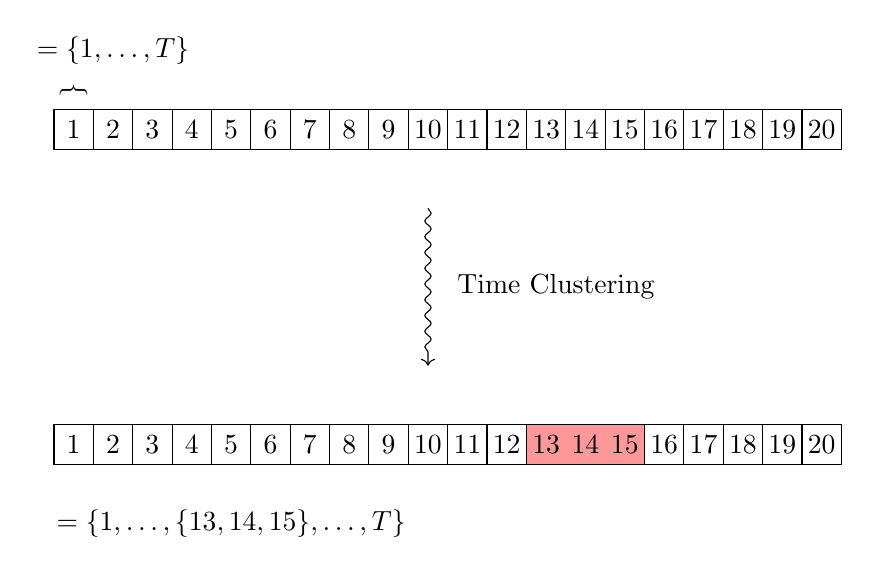
\begin{tikzpicture}
%draw first time partition
\nc{\step}{0.5}
\nc{\tblock}{+(-\step/2,-\step/2) rectangle ++(\step/2 + \step*0,\step/2)}
\draw (1,1) node{\(\cT = \{1, \ldots, T\}\)};
\foreach \x in {1,...,20}
  {
  \draw (\x*\step,0) \tblock;
  \draw (\x*\step,0) node{\x};
  }
\draw (\step,\step) node [rotate=-90] (BR) {\textbraceleft};

\draw [->,decorate,
decoration={snake,amplitude=.4mm,segment length=2mm,post length=1mm}]
(10*\step,-1 ) -- (10*\step,-3)
node [right,text width=3cm,align=center,midway]
{
Time Clustering 
};

\nc{\y}{-4}
\draw (2.5,\y-1) node{\(\cT = \{1, \ldots,\{13,14,15\},\ldots, T\}\)};
\foreach \x in {1,...,12}
  {
  \draw (\x*\step,\y) \tblock;
  \draw (\x*\step,\y) node{\x};
  }

\filldraw[fill=red!40,draw=black] (13*\step,\y) +(-\step/2,-\step/2) rectangle  ++(\step/2+\step*2,\step/2); %draw clustered time partitions
\draw (13*\step,\y) node{\(13\)};
\draw (14*\step,\y) node{\(14\)};
\draw (15*\step,\y) node{\(15\)};
\foreach \x in {16,...,20}
  {
  \draw (\x*\step,\y) \tblock;
  \draw (\x*\step,\y) node{\x};
  }
\end{tikzpicture}
\end{frame}


\section{Results}

\end{document}